\documentclass{article}
\usepackage{amsmath, amssymb, graphicx, geometry, tikz, array, booktabs, enumitem, listings, xcolor, fancyhdr, float, subcaption, hyperref}

\title{Module 5: Optimization and Gradient Descent}
\author{Machine Learning Course}
\date{}

\begin{document}

\maketitle
\tableofcontents
\newpage

% ---------------------------------------------------------
% Outline below is for reference only, not part of lecture
% ---------------------------------------------------------
% \section{Introduction}
\section{Introduction to Optimization in Machine Learning}

\subsection{The Optimization Framework}
In machine learning, we typically choose a model parameterized by $w$ by minimizing a loss function $L(w)$ that depends on the training data. This optimization problem is central to most machine learning algorithms.

\subsection{Common Loss Functions}
Different machine learning tasks use different loss functions:
\begin{itemize}
    \item \textbf{Linear Regression:}
    \[
    L(w) = \sum_{i=1}^{n} \left(y^{(i)} - w \cdot x^{(i)}\right)^{2}
    \]
    \item \textbf{Logistic Regression:}
    \[
    L(w) = \sum_{i=1}^{n} \ln \left(1 + e^{-y^{(i)}(w \cdot x^{(i)})}\right)
    \]
    where $y^{(i)} \in \{-1, 1\}$.
\end{itemize}

\subsection{Local Search Methods}
The default approach to solving these minimization problems is through local search:
\begin{enumerate}
    \item Initialize $w$ arbitrarily
    \item Repeat until convergence:
    \begin{enumerate}
        \item Find some $w'$ close to $w$ with $L(w') < L(w)$
        \item Move $w$ to $w'$
    \end{enumerate}
\end{enumerate}
Local search methods work particularly well when the loss function is convex, which we'll explore in detail later in this module.
% ...
% \section{Convexity}
\section{Convexity}

\subsection{Definition and Intuition}
A function $f: \mathbb{R}^d \rightarrow \mathbb{R}$ is convex if for all $a, b \in \mathbb{R}^d$ and $0 < \theta < 1$:
\[
f(\theta a + (1 - \theta) b) \leq \theta f(a) + (1 - \theta) f(b)
\]
Intuitively, this means that the line segment connecting any two points on the graph of the function lies above or on the graph.

\begin{figure}[h]
\centering
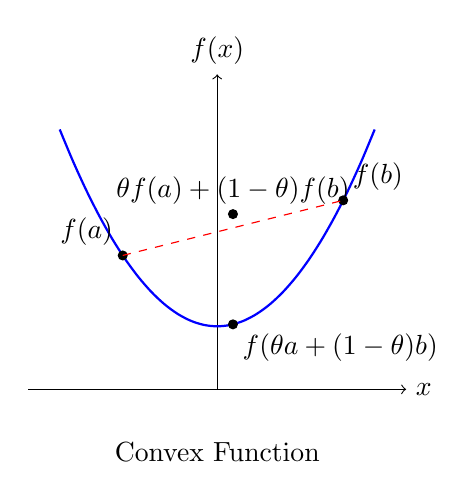
\begin{tikzpicture}[scale=0.8]
    % Convex function
    \draw[->] (-3,0) -- (3,0) node[right] {$x$};
    \draw[->] (0,0) -- (0,5) node[above] {$f(x)$};
    \draw[domain=-2.5:2.5, smooth, thick, blue] plot (\x, {(\x)^2/2 + 1});
    % Points and line segment
    \filldraw (-1.5, {(-1.5)^2/2 + 1}) circle (2pt) node[above left] {$f(a)$};
    \filldraw (2, {(2)^2/2 + 1}) circle (2pt) node[above right] {$f(b)$};
    \draw[red, dashed] (-1.5, {(-1.5)^2/2 + 1}) -- (2, {(2)^2/2 + 1});
    % Midpoint
    \filldraw (0.25, {(0.25)^2/2 + 1}) circle (2pt) node[below right] {$f(\theta a + (1-\theta)b)$};
    \filldraw (0.25, {0.25*(-1.5)^2/2 + 0.75*(2)^2/2 + 1}) circle (2pt) node[above] {$\theta f(a) + (1-\theta)f(b)$};
    \node at (0,-1) {Convex Function};
\end{tikzpicture}
\caption{Illustration of convexity: The function value at any point on the line segment connecting two points is less than or equal to the weighted average of the function values at those points.}
\end{figure}

A function is strictly convex if strict inequality holds for all $a \neq b$. Conversely, $f$ is concave if $-f$ is convex.

\subsection{Why Convexity Matters in Optimization}
Convexity ensures that any local minimum is a global minimum. This property is crucial for the success of local search and gradient-based optimization methods.

\subsection{Checking Convexity}
\subsubsection*{One Variable: Second Derivative Test}
A twice-differentiable function $f: \mathbb{R} \rightarrow \mathbb{R}$ is convex if and only if $f''(x) \geq 0$ for all $x$ in the domain.

\subsubsection*{Multivariate: Hessian and PSD Matrices}
For $f: \mathbb{R}^d \rightarrow \mathbb{R}$, the Hessian matrix $H(x)$ is defined as:
\[
H_{jk}(x) = \frac{\partial^2 f}{\partial x_j \partial x_k}(x)
\]
A twice-differentiable function is convex if and only if its Hessian is positive semidefinite (PSD) everywhere.

\subsection{Positive Semidefinite (PSD) Matrices}
A symmetric matrix $M$ is PSD if $x^T M x \geq 0$ for all $x \in \mathbb{R}^d$.

\textbf{Properties:}
\begin{itemize}
    \item Diagonal matrix is PSD if all diagonal entries $\geq 0$.
    \item If $M$ is PSD and $c > 0$, then $cM$ is PSD.
    \item If $M, N$ are PSD, then $M + N$ is PSD.
    \item $M$ is PSD iff $M = UU^T$ for some $U$.
    \item All covariance matrices are PSD.
\end{itemize}

\subsection{Worked Examples}

\paragraph{Example 1: Convexity of $f(x) = \|x\|^2$}
\[
f(x) = \|x\|^2 = \sum_{i=1}^d x_i^2
\]
\[
\frac{\partial f}{\partial x_j} = 2x_j
\]
\[
\frac{\partial^2 f}{\partial x_j \partial x_k} = 2\delta_{jk}
\]
So the Hessian is $2I$, which is positive definite. Therefore, $f(x)$ is strictly convex.

\paragraph{Example 2: Convexity of $f(z) = (u \cdot z)^2$}
\[
f(z) = (u \cdot z)^2
\]
\[
\frac{\partial f}{\partial z_j} = 2(u \cdot z)u_j
\]
\[
\frac{\partial^2 f}{\partial z_j \partial z_k} = 2u_j u_k
\]
So the Hessian is $2uu^T$, which is PSD since for any $x$, $x^T (2uu^T) x = 2(u^T x)^2 \geq 0$.

\paragraph{Example 3: Is $M = \begin{pmatrix} 1 & 1 \\ 1 & 1 \end{pmatrix}$ PSD?}
Let $x = (x_1, x_2)^T$:
\[
x^T M x = (x_1 + x_2)^2 \geq 0
\]
So $M$ is PSD.

\paragraph{Example 4: Is $M = \begin{pmatrix} 1 & 2 \\ 2 & 1 \end{pmatrix}$ PSD?}
Eigenvalues are $3$ and $-1$. Since one eigenvalue is negative, $M$ is not PSD.

\paragraph{Example 5: Convexity of Least Squares Loss}
\[
L(w) = \sum_{i=1}^n (y^{(i)} - w \cdot x^{(i)})^2
\]
The Hessian is $2\sum_{i=1}^n x^{(i)}(x^{(i)})^T$, a sum of PSD matrices, so $L$ is convex.

\paragraph{Example 6: Convexity of Logistic Regression Loss}
\[
L(w) = \sum_{i=1}^n \ln(1 + e^{-y^{(i)}(w \cdot x^{(i)})})
\]
Each term $\ell(z) = \ln(1 + e^{-z})$ has $\ell''(z) > 0$, so $L$ is convex.
% ...
% \section{Multivariate Differentiation}
\section{Multivariate Differentiation}

For $f: \mathbb{R}^d \to \mathbb{R}$:
\begin{itemize}
    \item \textbf{Gradient:} $\nabla f(w) = \left( \frac{\partial f}{\partial w_1}, \ldots, \frac{\partial f}{\partial w_d} \right)^T$
    \item \textbf{Hessian:} $H_{jk}(w) = \frac{\partial^2 f}{\partial w_j \partial w_k}$
\end{itemize}

\paragraph{Example 1: $F(w) = 3w_1w_2 + w_3$ for $w \in \mathbb{R}^3$}
\[
\frac{\partial F}{\partial w_1} = 3w_2, \quad \frac{\partial F}{\partial w_2} = 3w_1, \quad \frac{\partial F}{\partial w_3} = 1
\]
So,
\[
\nabla F(w) = (3w_2, 3w_1, 1)^T
\]

\paragraph{Example 2: $F(w) = w \cdot x$ where $x$ is fixed}
\[
\frac{\partial F}{\partial w_j} = x_j
\]
So,
\[
\nabla F(w) = x
\]

\paragraph{Example 3: Second Derivative Matrix of $F(w) = \|w\|^2$}
\[
F(w) = \sum_{j=1}^d w_j^2
\]
\[
\frac{\partial^2 F}{\partial w_j \partial w_k} = 2\delta_{jk}
\]
So the Hessian is $2I$.
% ...
% \section{Gradient Descent}
\section{Gradient Descent}

\subsection{The Gradient and Its Geometric Meaning}
The gradient points in the direction of steepest increase of a function. Moving in the negative gradient direction decreases the function most rapidly.

\subsection{Gradient Descent Algorithm}
\begin{enumerate}
    \item Initialize $w_0 = 0$, $t = 0$
    \item While $\|\nabla L(w_t)\| > \epsilon$ (not converged):
    \begin{enumerate}
        \item $w_{t+1} = w_t - \eta_t \nabla L(w_t)$
        \item $t = t + 1$
    \end{enumerate}
\end{enumerate}
Here, $\eta_t > 0$ is the step size (learning rate).

\subsection{Rationale: Local Linearity and Descent Direction}
For small $u$,
\[
L(w + u) \approx L(w) + u \cdot \nabla L(w)
\]
Choosing $u = -\eta \nabla L(w)$ for small $\eta$ ensures $L(w + u) < L(w)$.

\subsection{How to Set Step Size $\eta_t$?}
\begin{itemize}
    \item \textbf{Constant step size:} $\eta_t = \eta$
    \item \textbf{Diminishing step size:} $\eta_t = \frac{\eta_0}{1 + \beta t}$ or $\eta_t = \frac{\eta_0}{\sqrt{t}}$
    \item \textbf{Backtracking line search:} Iteratively decrease $\eta_t$ until $L(w_t - \eta_t \nabla L(w_t)) < L(w_t)$
    \item \textbf{Adaptive methods:} Adjust $\eta_t$ based on gradient history (e.g., AdaGrad, Adam)
\end{itemize}

\subsection{Gradient Descent for Logistic Regression: Full Derivation}
Given $(x^{(i)}, y^{(i)}) \in \mathbb{R}^d \times \{-1,1\}$,
\[
L(w) = \sum_{i=1}^n \ln(1 + e^{-y^{(i)}(w \cdot x^{(i)})})
\]
\begin{align}
\nabla L(w) &= \nabla \sum_{i=1}^{n} \ln(1 + e^{-y^{(i)}(w \cdot x^{(i)})}) \\
&= \sum_{i=1}^{n} \nabla \ln(1 + e^{-y^{(i)}(w \cdot x^{(i)})}) \\
&= \sum_{i=1}^{n} \frac{1}{1 + e^{-y^{(i)}(w \cdot x^{(i)})}} \cdot \nabla e^{-y^{(i)}(w \cdot x^{(i)})} \\
&= \sum_{i=1}^{n} \frac{1}{1 + e^{-y^{(i)}(w \cdot x^{(i)})}} \cdot e^{-y^{(i)}(w \cdot x^{(i)})} \cdot (-y^{(i)}x^{(i)}) \\
&= -\sum_{i=1}^{n} \frac{e^{-y^{(i)}(w \cdot x^{(i)})}}{1 + e^{-y^{(i)}(w \cdot x^{(i)})}} \cdot y^{(i)}x^{(i)} \\
&= -\sum_{i=1}^{n} \frac{1}{1 + e^{y^{(i)}(w \cdot x^{(i)})}} \cdot y^{(i)}x^{(i)} \\
&= -\sum_{i=1}^{n} P(Y \neq y^{(i)} | x^{(i)}, w) \cdot y^{(i)}x^{(i)}
\end{align}
Update rule:
\[
w_{t+1} = w_t - \eta_t \nabla L(w_t)
\]
% ...
% \section{Variants of Gradient Descent}
\section{Variants of Gradient Descent}

\subsection{Decomposable Loss Functions}
Many loss functions decompose as $L(w) = \sum_{i=1}^n \ell(w; x^{(i)}, y^{(i)})$.

\subsection{Stochastic Gradient Descent (SGD)}
Update using a single data point:
\[
w_{t+1} = w_t - \eta_t \nabla \ell(w_t; x^{(i)}, y^{(i)})
\]

\subsection{Mini-Batch Gradient Descent}
Update using a batch $B$:
\[
w_{t+1} = w_t - \eta_t \sum_{(x, y) \in B} \nabla \ell(w_t; x, y)
\]

\subsection{Comparison Table: GD, SGD, Mini-Batch GD}
\begin{table}[h]
\centering
\begin{tabular}{|l|l|l|l|}
\hline
\textbf{Method} & \textbf{Update Rule} & \textbf{Advantages} & \textbf{Disadvantages} \\
\hline
Gradient Descent & $w_{t+1} = w_t - \eta_t \nabla L(w_t)$ & 
Stable, accurate & Slow for large datasets, high memory \\
\hline
SGD & $w_{t+1} = w_t - \eta_t \nabla \ell(w_t; x^{(i)}, y^{(i)})$ & 
Fast, low memory, escapes local minima & Noisy, may not converge \\
\hline
Mini-Batch GD & $w_{t+1} = w_t - \eta_t \sum_{(x, y) \in B} \nabla \ell(w_t; x, y)$ & 
Balanced, parallelizable & Needs batch size tuning, still noisy \\
\hline
\end{tabular}
\caption{Comparison of gradient descent variants}
\end{table}
% ...
% \section{Convergence Properties}
\section{Convergence Properties}

\subsection{Convergence Guarantees for Convex Functions}
For convex $L(w)$ and appropriate step sizes, gradient descent converges to the global minimum.

\subsection{Rates for GD, SGD, and Accelerated Methods}
\begin{itemize}
    \item GD: $O(1/T)$ for general convex, linear for strongly convex.
    \item SGD: $O(1/\sqrt{T})$ in expectation.
    \item Accelerated (e.g., Nesterov): $O(1/T^2)$ for smooth convex.
\end{itemize}

\subsection{Practical Convergence Criteria (Stopping Conditions)}
\begin{itemize}
    \item $\|\nabla L(w_t)\| < \epsilon$
    \item $|L(w_{t+1}) - L(w_t)| < \delta$
    \item Maximum number of iterations
\end{itemize}
% ...
% \section{Advanced Optimization Methods}
\section{Advanced Optimization Methods}

\subsection{Momentum}
\[
v_{t+1} = \gamma v_t + \eta \nabla L(w_t)
\]
\[
w_{t+1} = w_t - v_{t+1}
\]
where $\gamma \in [0, 1)$.

\subsection{Adaptive Learning Rates}
\begin{itemize}
    \item AdaGrad: Per-parameter learning rates, decreases for frequent features.
    \item RMSProp: Exponential moving average of squared gradients.
    \item Adam: Combines momentum and RMSProp.
\end{itemize}

\subsection{Second-Order Methods}
\begin{itemize}
    \item Newton's Method: $w_{t+1} = w_t - [H(w_t)]^{-1} \nabla L(w_t)$
    \item Quasi-Newton (e.g., BFGS, L-BFGS): Approximate inverse Hessian.
\end{itemize}
% ...
% \section{Practical Considerations}
\section{Practical Considerations}

\subsection{Initialization Strategies}
\begin{itemize}
    \item For convex problems, any $w_0$ will converge.
    \item For non-convex (e.g., neural nets), initialization affects which minimum is found.
    \item Common: random, Xavier/Glorot, He initialization.
\end{itemize}

\subsection{Regularization and Its Effect}
Adding regularization (e.g., L2: $\lambda \|w\|^2$) can improve convexity and generalization.

\subsection{Non-Convex Optimization: Challenges and Context}
Many modern ML models (e.g., deep neural networks) are non-convex. While gradient descent can still work well in practice, there are no guarantees of finding the global minimum.

\subsection{Tips for Debugging and Tuning Optimization}
\begin{itemize}
    \item Monitor loss and gradients.
    \item Try different learning rates and batch sizes.
    \item Use validation data to check for overfitting.
    \item Visualize convergence when possible.
\end{itemize}
% ...
% \section{Summary and Key Takeaways}
\section{Practical Considerations}

\subsection{Initialization Strategies}
\begin{itemize}
    \item For convex problems, any $w_0$ will converge.
    \item For non-convex (e.g., neural nets), initialization affects which minimum is found.
    \item Common: random, Xavier/Glorot, He initialization.
\end{itemize}

\subsection{Regularization and Its Effect}
Adding regularization (e.g., L2: $\lambda \|w\|^2$) can improve convexity and generalization.

\subsection{Non-Convex Optimization: Challenges and Context}
Many modern ML models (e.g., deep neural networks) are non-convex. While gradient descent can still work well in practice, there are no guarantees of finding the global minimum.

\subsection{Tips for Debugging and Tuning Optimization}
\begin{itemize}
    \item Monitor loss and gradients.
    \item Try different learning rates and batch sizes.
    \item Use validation data to check for overfitting.
    \item Visualize convergence when possible.
\end{itemize}
% ...
\end{document}